
\section{Motivation}\label{sec:motivation}


In this section, we conduct a quantitative study  composed of several tests, in order
to deeply analyze the software tax that logging writes need to pay.
%We 
%conduct several tests with emulated logging writes.
The setup of our testing platform is detailed in Section \ref{sec:eval}.


\iftrue
\vspace{1ex}
\noindent\framebox[\columnwidth][s]{
	\parbox{\dimexpr\linewidth-2\fboxsep-2\fboxrule}{$\vmathbb{O1}$. \em
		%In the presence of device- and OS-level optimizations, 
		The  preallocation  strategy significantly
		boosts the performance of database logging writes. %write-intensive  workloads.
}}
\vspace{0.5ex}
\else
\ul{$\vmathbb{O1}$. \em
	%In the presence of device- and OS-level optimizations, 
	The  preallocation  strategy significantly
	boosts the performance of database logging writes. %write-intensive  workloads.
}
\fi

Database logging depends on   persistent file writes.
In the first test, we study an SSD (Samsung PM1725a)  which has supercapacitor-enabled PLP   and features low write latency. 
We use Fio~\cite{1fioFlex42:online} to create a file and repeatedly append data until it reaches 1GB, 
with 4KB per   request, each followed by   {fdatasync}. 
We configure two file creation options in Fio.
One preallocates a 1GB file at   start.
The other begins with an empty file that  grows to 1GB gradually. 
The file system is Ext4.
%TODO: DAC, MAC.
%, and we adhere to the default DAC for permission checks. 
This test aims to analyze the effect of  preallocation. 
%in the presence of advanced device- and OS-level optimizations.
%and 


\begin{figure}[!t]
	\centering
	\begin{subfigure}[t]{0.49\columnwidth}
		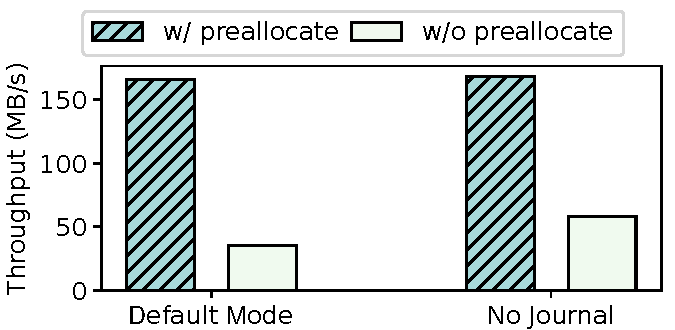
\includegraphics[width=\columnwidth, page=1]{./fig/mot/mot-preallocate.pdf}
		\caption{The Impact of Preallocation on File Writes.}
		\label{fig:Mot:mot-preallocate}
	\end{subfigure}
	\hfill
%	\begin{subfigure}[t]{0.75\columnwidth}
%	\includegraphics[width=\columnwidth, page=1]{fig/mot/mot-breakdown-legend.pdf}
%\end{subfigure}	
	\begin{subfigure}[t]{0.49\columnwidth}
	 	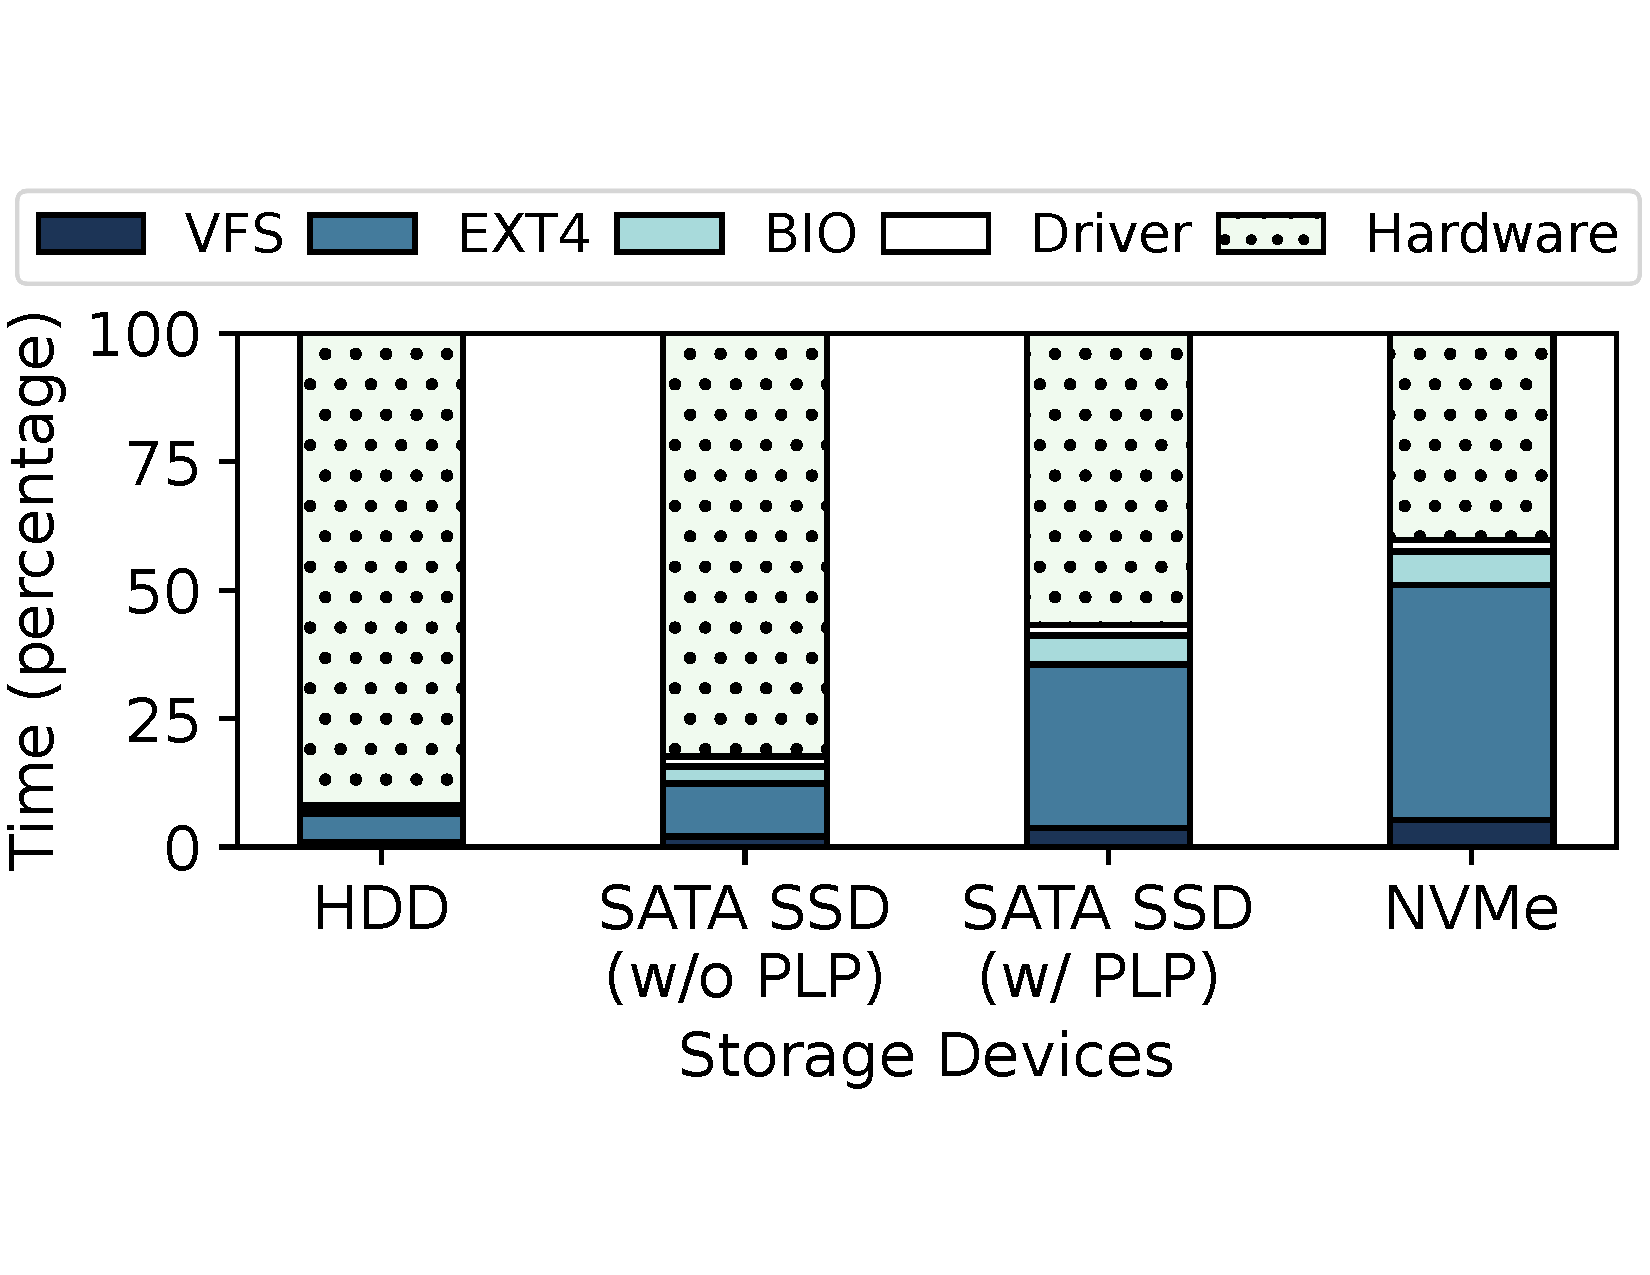
\includegraphics[width=\columnwidth, page=1]{fig/mot/mot-breakdown2.pdf} 
		\caption{The Breakdowns  on the File I/O Path.}
		\label{fig:Mot:workload-breakdown}
	\end{subfigure}
	\vspace{-0.5ex}
	\caption{The Impact of Preallocation on File Writes and the Breakdowns on the File I/O Path with Varying Devices.}
	\vspace{-2ex}
\end{figure}


\autoref{fig:Mot:mot-preallocate} shows the throughput (bandwidth in MB/s) 
for writing data to two files when Ext4 is mounted in two modes. 
%Let us first take for illustration 
In the default \texttt{data=ordered} mode,  
%In this mode, 
the   throughput increases from 35MB/s to 166MB/s.
%
%As illustrated in , preallocation yields dramatic improvements on an NVMe SSD (Samsung PM1725a), increasing throughput from 35MB/s to 166MB/s under Ext4's default {\tt data=ordered} mode. 
%This 4.7$\times$ improvement mainly stems from eliminating the cost of
This improvement occurs because preallocation eliminates on-demand block allocation 
and avoids metadata journaling. %~\cite{lee2015waldio}.
%
%
Comparatively, for the growing file,
%%%In the meantime,
%However, the stark performance gap reveals a critical issue: 
%%%appending data to a
%%%dynamically growing file % are widely used in production systems, but
%%%suffers from severe overheads. In this test, 
each appending write   triggers a cascade of  operations on the critical path, including the query of block groups for free space,
%extent tree updates, 
%block group searches, 
the modification of block bitmap upon allocation,  the update of file's extent tree, 
and the composition and commit of metadata changes to the journal.
%bitmap modifications, and journal commits. 
These operations   construct a serious performance cost that becomes increasingly problematic with fast storage devices like the  SSD we are using.
%Also, preallocation relieves the  classic double logging issue \cite{huang2022removing,10.1145/2897073.2897093,lee2015waldio}. % is also relieved.
% during writes to a fixed-size file. In other words, this optimization solves the double-logging database problem\cite{huang2022removing}.
Even if we disable   journaling, i.e., `No Journal' in \autoref{fig:Mot:mot-preallocate},
preallocation still yields   significant performance improvements. Additionally, 
%contiguous   blocks are likely to be assigned to a preallocated   file, 
preallocation is likely to ask Ext4 to assign contiguous blocks to a file,
which is
 beneficial for the sequential appending I/O pattern of database logging. 
%On the other hand, a comparison between results obtained with {\tt data=ordered} and no journal modes
%indicates that,
%%regardless of journaling or not, the preallocation yields high and stable throughput.
%, while disabling the journaling with a risk of inconsistent metadata just gains moderate performance improvement.
% the throughput remains stable for the preallocated file as preallocation helps to avoid metadata change or journaling, while
%the throughput for the growing file increases by 50.7\% with the journaling disabled.
%Regardless of journaling or not, the pre-initialization of a file's structure through preallocation
% the throughput of appending data to the growing file
% increases by \todo{xx}\%.
%This indicates th
To sum up,
 {\em we shall adopt the preallocation-like strategy 	to better exploit the	device- and OS-level optimizations
for accelerating   logging writes}.

\iftrue
\vspace{1ex}
\noindent\framebox[\columnwidth][s]{
\parbox{\dimexpr\linewidth-2\fboxsep-2\fboxrule}{$\vmathbb{O2}$. \em
%With preallocated files and PLP-enabled SSDs, traditional filesystem and VFS overheads become the dominant performance bottleneck.
%Despite the use  of preallocation and low-latency SSD, the 
The   software tax is dominated by file system operations  and badly
impairs the performance of database logging.}
}
\vspace{0.5ex}
\else
\ul{$\vmathbb{O2}$. \em
	%With preallocated files and PLP-enabled SSDs, traditional filesystem and VFS overheads become the dominant performance bottleneck.
%	Despite the use  of preallocation and low-latency SSD, the runtime software tax dominated by file system operations   badly
%	impairs the performance of database logging.
The runtime software tax is dominated by file system operations  and badly
impairs the performance of  logging.
}
\fi

We next assess the  software tax imposed per   write with a preallocated file.
%In the second test, 
We use four   devices for a comprehensive analysis:
 %in the second test. 
%
%To assess the software tax with varying storage devices,
%we perform tests on four devices with increasing performance capabilities: 
a   hard disk (WDC WD20EZWX), a SATA SSD without PLP (Samsung 870EVO), a SATA SSD with PLP (Samsung PM893), and an  NVMe SSD with PLP (Samsung PM1725a). 
We measure  the time cost of each software layer   using Intel VTune Profiler \cite{GetStart56:online}. 
The I/O pattern is the same   as used in the first test with a preallocated file under Ext4 file system.
%The file system is Ext4 
%({\tt data=ordered}).
\autoref{fig:Mot:workload-breakdown} presents the breakdowns for hardware and software layers with four devices.
%Results depicted in \autoref{fig:Mot:workload-breakdown} 
In spite of  preallocation, {\em the runtime
	software tax increasingly dominates   I/O latency
	as   devices become faster}, reaching  60.2\% for the   NVMe SSD. 


%\textbf{Preallocated files shift the bottleneck.} 
%When using preallocated files—a common optimization in commercial databases—the traditional bottlenecks of dynamic block allocation and filesystem journaling are largely eliminated.
%We have deeply studied what layers determine the software tax with regard to the use of preallocation and PLP.
% with regard to writing data in the presence of preallocation and PLP.
 %Our profiling reveals that with preallocation and PLP, the software overhead composition fundamentally changes: 
%In all software cost, VFS  operations account for 23.1\%, file system operations consume 46.3\%, and I/O scheduling contributes 24.8\%. 
Specifically,
%as shown in \autoref{fig:Mot:workload-breakdown}, 
% we find that
  Ext4 % file system
   is the predominant latency
source with the NVMe SSD, contributing about 46.3\%. % as shown in \autoref{fig:Mot:workload-breakdown}. % of the total software overhead. 
%Although preallocation and fdatasync minimize the cost of  journaling, 
 Although no structural change occurs to the file,
  frequent metadata operations persist, mainly due to searching
  for target block numbers
   in the
per-file mappings \cite{SSD:BypassD:ASPLOS-2024}.
%and permission checks. 
{\em Moving such search operations off the critical path shall effectively
reduce the overall software tax}.
%%%, thereby underscoring the necessity of software stack refinements especially for preallocated log files.
% Notably, even with preallocation, residual metadata operations for permission checks, extent validation, and file mapping persist, contributing significant overhead that was previously masked by more expensive allocation operations.

\iftrue
\vspace{1ex}
\noindent\framebox[\columnwidth][s]{
\parbox{\dimexpr\linewidth-2\fboxsep-2\fboxrule}{$\vmathbb{O3}$. \em
For non-preallocated log files, logging writes still incur severe  overhead, which  can be mitigated through a preallocation-like strategy.}
}
\vspace{0.5ex}
\else
\ul{$\vmathbb{O3}$. \em
	For non-preallocated log files, logging writes incur severe  overhead, which  can be mitigated through a preallocation-like strategy.}
\fi
%In many real-world production environments, 
%such as some databases like MySQL \cite{mysql-binlog},
%such as scientific computing and streaming analytics \cite{spark-streaming},

\begin{comment}
: %, which is briefly described as follows.
%, severely impacting performance. 
%To understand this overhead, we first examine Ext4's preallocation mechanism. 
before accepting data for the target file,
%When a file expands before accepting data, %grows % an append operation, 
Ext4 asks for new blocks from the block group(s), updates the file's extent trees, and commits these metadata changes into the
 journal  for crash consistency. 
\end{comment}

\begin{figure}[!t]
\centering
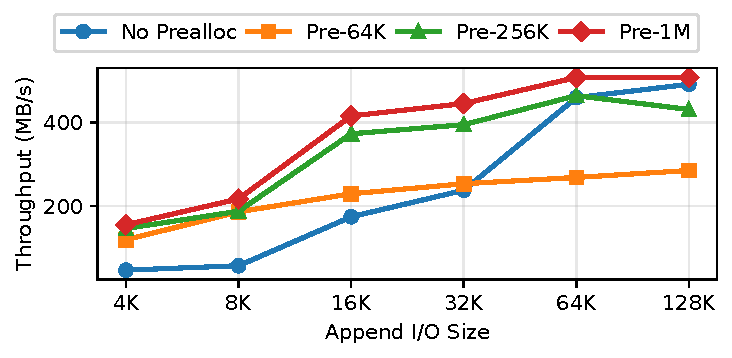
\includegraphics[width=0.9\columnwidth]{fig/mot/prealloc_throughput.pdf}
%\caption{Impact of step-wise preallocation on throughput for different append I/O sizes.}
\vspace{-1ex}
\caption{The Impact of On-the-fly Preallocation on Appending Writes on a Dynamically Growing File.}
\label{fig:mot:prealloc-throughput}
\vspace{-4ex}
\end{figure}

Real-world databases may  use preallocated or growing log files, % without preallocation,
 such as the binlog  of MySQL \cite{mysql2013mysql}.
%appending data to a   growing file, such as the binary log (binlog) file used by MySQL \cite{mysql-binlog},
% is   widely used  alongside preallocating a large file in advance.
%Many real-world environments, 
%The previous analysis focused on fully preallocated files, a common optimization in commercial databases. However, many production scenarios cannot leverage full preallocation—log rotation policies \cite{rotatelogs}, streaming analytics \cite{spark-streaming}, and unpredictable workloads in distributed systems \cite{kafka-log} all require dynamically growing files. 
%In these cases, each
As mentioned,
an appending write triggers costly runtime operations with   a growing file.
We investigate if there is a chance that we can accelerate file  writes issued to non-preallocated log files 
in a preallocation-like way.
In the third test, 
we append overall 10GB data to a file in the direct I/O mode %TODO: do you call fdatasync -- wangc@2025.09.13-16:59
with the size per write being
4KB, 8KB, 16KB, 32KB, 64KB, and 128KB. They cover common database transaction sizes for logging
in practice.
We primarily create an empty file to complete this appending task.
The curve with dots in \autoref{fig:mot:prealloc-throughput} 
shows a rising throughput 
with the increase of I/O size. 
Next, we explicitly apply an on-the-fly  preallocation prior to each appending write. That is, we call fallocate to 
%extend the file's capacity 
preallocate numerous blocks to the file
 %by some blocks 
 before   appending data. Without loss of generality,
we extend the file in 64KB, 256KB, or 1MB at a time. We 
  initialize  preallocated blocks by filling zeros after      fallocate %syscall
to truly acquire the  space and invoke fsync to trigger journaling in advance. % as well.
By doing so, we intend to concretely prepare space  in a batched manner for one or multiple subsequent 
appending writes.
%to extend the file 
%we  quantitatively 
%Regarding the aforementioned effect of preallocation, we consider if we can emulate a preallocation-like
%way 

\begin{table}[!t]
	\centering
	{\large
		\renewcommand{\arraystretch}{1.3}%  ← row spacing factor
		\caption{A Comparison between SOTA Designs.}
		\label{tab:mot:sota-comparison}
			\vspace{-1ex}
		\begin{adjustbox}{max width=0.5\textwidth}
			%\begin{tabular}{*{6}{c}} 
			\begin{tabular}{lcccccc} 	
				\toprule
			Solutions	& \multicolumn{1}{c}{\makecell{No\\ hardware\\change}} 
				& \multicolumn{1}{c}{\makecell{Non-\\intrusive\\kernel}} 
				& \multicolumn{1}{c}{\makecell{Transparent\\support for\\applications}} 
				& \multicolumn{1}{c}{\makecell{Existing\\file system\\compatibility}} 
				& \multicolumn{1}{c}{\makecell{Compati- \\ bility  with  \\SATA SSD}} \\
				\midrule
				SPDK     & \checkmark & \checkmark & $\times$   & $\times$   & \checkmark  \\
				NVMeDirect & \checkmark & $\times$  & $\times$   & $\times$   & $\times$ \\
				Moneta-D   & $\times$   & $\times$  & \checkmark & \checkmark & \checkmark \\
				BypassD   & $\times$   & $\times$  & \checkmark & \checkmark & $\times$ \\
				\textcolor{blue}{\bf \odes} & \textcolor{blue}{\bf \Checkmark} & \textcolor{blue}{\bf \Checkmark} & \textcolor{blue}{\bf \Checkmark} & \textcolor{blue}{\bf \Checkmark} & \textcolor{blue}{\bf \Checkmark} \\
				\bottomrule
			\end{tabular}
		\end{adjustbox}
	}
	\vspace{-3ex}
\end{table}

In \autoref{fig:mot:prealloc-throughput},
the other 
three curves with squares, triangles, and diamonds represent the bandwidths
with dynamically preallocating 64KB, 256KB, and 1MB, respectively.
A comparison among four curves brings about two inspiring points.
%, we can obtain two inspiring points.
First, {\em  on-the-fly preallocation, though incurring allocation and journaling overheads on the critical path, is likely to boost   write performance}.
For example, given the typical I/O size of 4KB, the throughput increases by 2.6$\times$, 3.2$\times$, and 3.4$\times$
with three spaces  allocated ahead, 
respectively. Note that 
preallocating a contiguous space causes file system  journaling once, whose cost
%and this cost 
is much less than the accumulated cost of journaling for every small   write.
Secondly, {\em the effect of on-the-fly preallocation diminishes when the I/O size is close to or   greater
than the preallocation size}. A large I/O   itself will trigger   space allocation, and
preallocating space  turns to be neither necessary nor meaningful.
%, but adversely incurs extra overhead as a side effect.

Furthermore, we have thought about what % we
%this test and results   what 
we can do to improve beyond this test. 
Although {\em on-the-fly preallocation is effective when combining smaller writes with larger allocated space}, 
{\em Ext4 introduces substantial time cost for each allocation on the critical path} due to  space management and metadata journaling.
% {\em   Ext4 file system imposes   heavy software tax for each preallocation on the critical path}. 
Our design must address this issue (see Section~\ref{sec:design}).
% will be addressed with our design in the next section.
%
%the journaling cost for every small appending writes.

 %TODO: a reference here. -- wangc@2025.09.13-16:19.
\begin{comment}
	Moreover,   uninitialized blocks shall be initialized 
	upon the factual write, 
	incurring additional cost. % updates.
\end{comment}


%To reduce the jbd2 overhead from append I/O operations, we employ a step-wise preallocation strategy that reserves space in advance, thereby reducing the frequency of jbd2 transaction invocations from every append to only when new space needs to be allocated. We conducted experiments using O\_DIRECT to bypass the page cache and isolate storage behavior on an NVMe SSD (Samsung PM1725a), writing 10GB total data with varying append sizes and preallocation strategies. The x-axis shows append I/O sizes from 4KB to 128KB, while the y-axis shows throughput in MB/s. Each line represents a different preallocation strategy: 0K indicates traditional append-only writes without any preallocation (baseline), where every append triggers jbd2 journaling; 64K means preallocating 64KB chunks—when the current preallocated space is exhausted by append writes, the next 64KB is preallocated via \texttt{fallocate}; similarly, 256K and 1M represent preallocating 256KB and 1MB chunks respectively. Our test explicitly converts uninitialized extents to initialized by writing zeros after each \texttt{fallocate}.

\begin{comment}


As shown in \autoref{fig:mot:prealloc-throughput}, the results reveal stark performance differences. For 4KB appends without preallocation (0K baseline), throughput is only 46.3 MB/s—each append triggers a jbd2 transaction for metadata updates. With 1MB step-wise preallocation, 4KB appends achieve 155.2 MB/s, a 3.4× improvement. This dramatic gain stems from amortizing jbd2 overhead: instead of journaling every 4KB append, metadata updates occur only every 1MB. However, larger append sizes show diminishing returns from preallocation. For 128KB appends, throughput improves modestly from 491.7 MB/s (baseline) to 508.1 MB/s (1MB prealloc)—only 3.4\% gain. This occurs because the relative cost of journaling per byte written decreases as append size increases. And the step-wise preallocation also introduces overhead on the critical path. Each \texttt{fallocate} call and subsequent initialization with zeros adds synchronous latency—for 1MB preallocation. While beneficial for small appends where jbd2 dominates, this overhead becomes proportionally significant for large appends where data movement already dominates. These findings motivate \odes's design optimizations: we employ asynchronous preallocation and initialization off the critical path, allowing small appends to benefit from reduced jbd2 overhead without penalizing large append performance.
\end{comment}


\iftrue
\vspace{1ex}
\noindent\framebox[\columnwidth][s]{
\parbox{\dimexpr\linewidth-2\fboxsep-2\fboxrule}{$\vmathbb{O4}$. \em
State-of-the-art solutions developed to reduce the software tax exhibit considerable limitations.}
}
\vspace{0.5ex}
\else 
\ul{$\vmathbb{O4}$. \em
	SOTA designs targeting the software tax have   limitations.}
\fi

Regarding the  evolution of storage devices,
researchers have studied the  software tax charged on file I/Os. % have to pay.
\autoref{tab:mot:sota-comparison} shows   state-of-the-art (SOTA) solutions in five dimensions. Intel
SPDK~\cite{SSD:SPDK:CloudCom-2017} and NVMeDirect  \cite{SSD:NVMeDirect:HotStorage-2016}  demand 
extensive reprogramming efforts  due to poor POSIX API compatibility, challenging the reliance of databases on standard file I/O interfaces.  %Comparatively,
Moneta-D \cite{SSD:Moneta-D:ASPLOS-2012} and BypassD~\cite{SSD:BypassD:ASPLOS-2024} are more compatible
with existing file systems and   databases. Nevertheless, they  require kernel changes and/or specialized hardware or 
software. %Let us
Take BypassD for illustration. It handles a request of mapping an in-file offset to  target block number through
a specialized IOMMU. Also, its implementation introduces more than 4,200 lines of code (LOC) in the Linux kernel.
 %such as enhanced IOMMU and 
  Furthermore, it only supports NVMe SSD.
 These
hinder its portability and usability. 
In all,
such drawbacks   limit the effectiveness of SOTA designs in general-purpose  production environments.




\begin{comment}
 

To address these challenges, we introduce \odes, an all-in-software solution that eliminates software tax for both preallocated and dynamically growing files. \odes decouples I/O operations from file management through eBPF-based interception and direct device access. For dynamically growing files, \odes employs an innovative donor-based allocation strategy using Ext4's \texttt{move\_extent} feature, enabling efficient block management without repeated journaling overhead. This approach preserves POSIX compatibility and access protection while facilitating seamless integration into existing database systems, remaining compatible with both SATA and NVMe SSDs.
\end{comment}